\chapter{Termodinámica estadística: funciones de partición}\label{ch:b3:partition-functions}

La tumba de Ludwig Boltzmann en Viena lleva una sola línea, $S = k\log W$: la
entropía de un sistema cuenta las maneras en que sus moléculas pueden repartirse su energía.
La termodinámica, tal como la construyeron los volúmenes del primer y del segundo año, nunca necesita
las moléculas: relaciona entre sí calores medidos, entropías y constantes de equilibrio.
La termodinámica estadística los calcula a partir de las propias
moléculas. Su objeto central es una sola suma sobre los niveles de energía de una
molécula, la función de partición; los niveles proceden de la espectroscopia, y la
entropía estándar del nitrógeno calculada a partir de su espectro concuerda con el
valor tabulado hasta la centésima de julio por kelvin y por mol. Este capítulo
construye la función de partición, la separa en sus partes de traslación, rotación,
vibración y electrónica, y la convierte en energía interna, entropía
y energía de Gibbs; el \cref{ch:b3:statistical-thermo-applied} la aplica a las capacidades
caloríficas y a las constantes de equilibrio.

\begin{recall}
El volumen del segundo año definió la entropía molar estándar, la energía de Gibbs y el
potencial químico, y tabuló entropías obtenidas a partir de capacidades caloríficas
medidas hasta bajas temperaturas. El \cref{ch:b3:quantum-model-systems} dio los
niveles de energía de una \omterm{def:b3:quantum-model-systems:box}{partícula en una caja}, del \omterm{def:b3:quantum-model-systems:oscillator}{oscilador armónico} y del
\omterm{def:b3:quantum-model-systems:rotor}{rotor rígido}, $E_J = hcBJ(J+1)$ con \omterm{def:b3:quantum-model-systems:degenerate}{degeneración} $2J + 1$; el
\cref{ch:b3:rovibrational-spectroscopy} midió $B$ y $\tilde\nu$ para moléculas
diatómicas y encontró que, en una molécula homonuclear como \ce{N2}, los
espines nucleares hacen desiguales los niveles de rotación alternos.
\end{recall}

\section{Microestados y distribución de Boltzmann}

Sean $N$ moléculas idénticas e independientes que pueden ocupar niveles de energía
$\varepsilon_0 = 0 < \varepsilon_1 < \varepsilon_2 < \dots$, con energía total $E$. Decir cuántas
moléculas hay en cada nivel, $\{n_0, n_1, \dots\}$, describe una distribución;
decir qué molécula está en qué nivel describe mucho más.

\begin{definition}[Microestado, peso estadístico]\label{def:b3:partition-functions:microstate}
Un \emph{microestado}\index{microestado} de un sistema de moléculas es una especificación
completa del estado de cada molécula. El \emph{peso
estadístico}\index{peso estadistico@peso estadístico} $W$ de una distribución $\{n_i\}$ de $N$ moléculas sobre
niveles no degenerados es el número de microestados que la realizan:
\[
  W = \frac{N!}{n_0!\,n_1!\,n_2!\cdots}.
\]
\end{definition}

\begin{example}[Tres cuantos entre tres osciladores]\label{ex:b3:partition-functions:three-quanta}
Tres osciladores comparten tres cuantos de energía. La distribución ``un
oscilador tiene los tres'' puede realizarse de $3!/(1!\,2!) = 3$ maneras, ``uno
tiene dos y otro uno'' de $3! = 6$ maneras y ``cada uno tiene uno'' de una sola manera:
diez \omterm{def:b3:partition-functions:microstate}{microestados} en total, y la distribución más uniforme que aún reparte la
energía sobre varios niveles es la más probable. Con $10^{23}$ moléculas, los
pesos se vuelven tan picudos que una distribución, y las que difieren
de ella en una cantidad despreciable, reúnen prácticamente todos los \omterm{def:b3:partition-functions:microstate}{microestados}.
\end{example}

\begin{remark}
El postulado de la termodinámica estadística es que todos los \omterm{def:b3:partition-functions:microstate}{microestados} de un
sistema aislado con una energía dada son igualmente probables. El sistema se
encuentra entonces, de forma abrumadora, en la distribución de mayor peso: encontrarla es la
tarea de esta sección.
\end{remark}

Para números grandes, la aproximación de Stirling $\ln x! \approx x\ln x - x$ da
\[
  \ln W = N\ln N - \sum_i n_i\ln n_i .
\]

\begin{definition}[Distribución de Boltzmann, población]\label{def:b3:partition-functions:boltzmann}
La \emph{población}\index{poblacion@población} $n_i/N$ de un nivel es la fracción de las
moléculas que lo ocupan. La \emph{distribución de Boltzmann}\index{distribucion de Boltzmann@distribución de Boltzmann}
es la distribución de mayor peso de unas moléculas independientes en
equilibrio térmico a la temperatura $T$, dada por el teorema siguiente.
\end{definition}

\begin{theorem}[La distribución de Boltzmann]\label{thm:b3:partition-functions:boltzmann}
Para moléculas independientes en equilibrio a la temperatura $T$, la \omterm{def:b3:partition-functions:boltzmann}{población} de un
nivel de energía $\varepsilon_i$ y \omterm{def:b3:quantum-model-systems:degenerate}{degeneración} $g_i$ es
\[
  \frac{n_i}{N} = \frac{g_i\eu^{-\varepsilon_i/kT}}{q},
  \qquad q = \sum_i g_i\eu^{-\varepsilon_i/kT},
\]
donde $k$ es la constante de Boltzmann. Dos niveles tienen \omterm{def:b3:partition-functions:boltzmann}{poblaciones} en la razón
$\frac{n_j}{n_i} = \frac{g_j}{g_i}\eu^{-(\varepsilon_j - \varepsilon_i)/kT}$.
\end{theorem}

\begin{proof}[Demostración parcial]
Se toman primero niveles no degenerados. Se maximiza $\ln W$ con las dos restricciones
$\sum_in_i = N$ y $\sum_in_i\varepsilon_i = E$, con multiplicadores de Lagrange $\alpha$ y $\beta$:
para todo $i$,
\[
  \frac{\partial}{\partial n_i}\Bigl(\ln W + \alpha\sum_jn_j - \beta\sum_jn_j\varepsilon_j\Bigr)
  = -\ln n_i - 1 + \alpha - \beta\varepsilon_i = 0,
\]
luego $n_i = \eu^{\alpha - 1}\eu^{-\beta\varepsilon_i}$, y la primera restricción fija $\eu^{\alpha - 1}
= N/\sum_j\eu^{-\beta\varepsilon_j}$. Un nivel de \omterm{def:b3:quantum-model-systems:degenerate}{degeneración} $g_i$ son $g_i$ estados distintos de
la misma energía, cada uno poblado como arriba: su \omterm{def:b3:partition-functions:boltzmann}{población} se multiplica por
$g_i$. El multiplicador $\beta$ se identifica con un caso conocido: para el
movimiento de traslación de un gas ideal (\cref{prop:b3:partition-functions:q-trans}
más abajo), la distribución da una energía $\frac32N/\beta$, y la energía del gas
ideal es $\frac32NkT$; por tanto, $\beta = 1/kT$. Que $\beta$ sea la misma magnitud para todo
tipo de movimiento, y que sea la temperatura termodinámica, se admite
aquí: dos sistemas en contacto térmico comparten el mismo $\beta$, que es la propiedad que
define la temperatura.
\end{proof}

\begin{definition}[Función de partición molecular]\label{def:b3:partition-functions:partition-function}
La \emph{función de partición molecular}\index{funcion de particion molecular@función de partición molecular} de una
molécula a la temperatura $T$ es la suma
\[
  q = \sum_{\text{niveles}}g_i\eu^{-\varepsilon_i/kT} = \sum_{\text{estados}}\eu^{-\varepsilon_s/kT},
\]
con las energías medidas desde el nivel más bajo, de modo que $q \ge 1$.
\end{definition}

La función de partición cuenta los estados que son térmicamente accesibles: a
temperatura muy baja solo contribuye el nivel más bajo y $q \to g_0$; a temperatura
muy alta cada estado contribuye con alrededor de 1 y $q$ crece sin límite.
De ahí una regla práctica: los niveles situados mucho más de $kT$ por encima del más bajo están
vacíos; los niveles situados a menos de $kT$ de él están poblados. A \qty{298.15}{K}, $kT$ corresponde
a \qty{207.2}{cm^{-1}}, o $RT = \qty{2.479}{kJ/mol}$.

\begin{method}[Poblaciones de los niveles a partir de las constantes espectroscópicas]\label{met:b3:partition-functions:populations}
\begin{enumerate}
  \item Enumerar los niveles con sus energías (a partir de las constantes, p.~ej.,
        $hcBJ(J+1)$) y sus \omterm{def:b3:quantum-model-systems:degenerate}{degeneraciones} ($2J + 1$).
  \item Expresar cada energía en unidades de $kT$; a \qty{298.15}{K}, dividir un
        número de onda por \qty{207.2}{cm^{-1}}.
  \item Formar los términos $g_i\eu^{-\varepsilon_i/kT}$, sumarlos para obtener $q$ y dividir.
        Detener la suma cuando los términos sean despreciables.
  \item Comprobar: las \omterm{def:b3:partition-functions:boltzmann}{poblaciones} suman 1; la razón entre dos de ellas es
        $\frac{g_j}{g_i}\eu^{-(\varepsilon_j-\varepsilon_i)/kT}$.
\end{enumerate}
\end{method}

\begin{example}[Los niveles de rotación del cloruro de hidrógeno]\label{ex:b3:partition-functions:hcl}
% ledger: diat:HCl.Be, diat:HCl.ae
Para \ce{H^{35}Cl}, $B_0 = B_e - \alpha_e/2 = \qty{10.44}{cm^{-1}}$. A \qty{300}{K}, el nivel $J$
está a $10.44\,J(J+1)$~\unit{cm^{-1}}, es decir, a $0.0501\,J(J+1)$ en unidades de $kT$. Los términos
$(2J+1)\eu^{-0.0501J(J+1)}$ valen 1, 2.71, 3.70, 3.84, 3.31, 2.45, \dots; su suma es
$q = 20.3$ y las \omterm{def:b3:partition-functions:boltzmann}{poblaciones} de $J = 0$ a 4 son 0.049, 0.134, 0.182, 0.189 y
0.163: el nivel más poblado es $J = 3$, no $J = 0$, porque la \omterm{def:b3:quantum-model-systems:degenerate}{degeneración}
$2J + 1$ crece mientras el factor de Boltzmann disminuye. Es la envolvente de la
banda de rotación--vibración del \cref{ch:b3:rovibrational-spectroscopy}.
\end{example}

\begin{omfigure}
\begin{tikzpicture}[font=\small]
  % levels J = 0-3, g = 2J+1, energies 0, 1, 3, 6 (units of 2hcB); bars = 3.5 cm x population
  % of the four levels alone at kT = 2hcB (0.422, 0.466, 0.105, 0.007) and kT = 10hcB (0.120, 0.296, 0.330, 0.254)
  \foreach \J/\e/\g/\lo/\hi in {0/0/1/1.48/0.42, 1/1/3/1.63/1.04, 2/3/5/0.37/1.16, 3/6/7/0.03/0.89}{
    \draw[thick] (0,0.55*\e) -- (2.2,0.55*\e);
    \node[anchor=east] at (0,0.55*\e) {$J = \J$};
    \node[anchor=west, font=\scriptsize] at (2.25,0.55*\e) {$g = \g$};
    \fill[omDef!70] (3.4,0.55*\e-0.11) rectangle ++(\lo,0.22);
    \fill[omThm!70] (6.4,0.55*\e-0.11) rectangle ++(\hi,0.22);
  }
  \node[anchor=south, omDef] at (4.2,3.6) {$T$ baja};
  \node[anchor=south, omThm] at (7.2,3.6) {$T$ alta};
  \draw[->] (-1.4,0) -- (-1.4,3.7) node[anchor=south] {$\varepsilon$};
\end{tikzpicture}

{\small Una escalera de Boltzmann: niveles de rotación $J = 0$ a 3 (energías $0$, $2$, $6$,
$12$ veces $hcB$, \omterm{def:b3:quantum-model-systems:degenerate}{degeneraciones} $2J + 1$) y sus \omterm{def:b3:partition-functions:boltzmann}{poblaciones}, como longitudes de barras,
a $kT = 2hcB$ y $kT = 10hcB$ (solo los cuatro niveles). Al calentar, el nivel más bajo se
vacía hacia los superiores; a ambas temperaturas las barras suman
el mismo total, el número de moléculas.}
\end{omfigure}

\section{La función de partición molecular}

\begin{proposition}[Factorización]\label{prop:b3:partition-functions:factorisation}
Si la energía de una molécula es una suma de contribuciones independientes,
$\varepsilon = \varepsilon^{\mathrm T} + \varepsilon^{\mathrm R} + \varepsilon^{\mathrm V} + \varepsilon^{\mathrm E}$, siendo cada estado
cualquier combinación de un estado de traslación, uno de rotación, uno de vibración y uno
electrónico, entonces
\[
  q = q^{\mathrm T}q^{\mathrm R}q^{\mathrm V}q^{\mathrm E}.
\]
\end{proposition}

\begin{proof}
La suma sobre todas las combinaciones de una exponencial de una suma es el producto de las
sumas separadas: $\sum_{a,b}\eu^{-(\varepsilon_a+\varepsilon_b)/kT} = \bigl(\sum_a\eu^{-\varepsilon_a/kT}\bigr)
\bigl(\sum_b\eu^{-\varepsilon_b/kT}\bigr)$, y lo mismo para cuatro factores.
\end{proof}

La separación es una aproximación: la rotación y la vibración interaccionan (la
constante $\alpha_e$), y el estado electrónico fija las \omterm{def:b3:rovibrational-spectroscopy:rotational-constant}{constantes de rotación} y de vibración.
Para una molécula en su estado electrónico fundamental a temperaturas
ordinarias, los errores son de unas centésimas de julio por kelvin en una
entropía. Las \omterm{def:b3:partition-functions:boltzmann}{poblaciones} se calculan entonces por separado para cada tipo de movimiento:
la fracción de moléculas en un nivel de vibración $v$ no depende de su
rotación.

\section{Las cuatro contribuciones}

\subsection*{Traslación}

\begin{definition}[Longitud de onda térmica]\label{def:b3:partition-functions:thermal-wavelength}
La \emph{longitud de onda térmica}\index{longitud de onda termica@longitud de onda térmica} de una molécula de masa $m$ a la
temperatura $T$ es $\Lambda = \dfrac{h}{\sqrt{2\pi mkT}}$.
\end{definition}

\begin{proposition}[Función de partición de traslación]\label{prop:b3:partition-functions:q-trans}
Para una molécula de masa $m$ que se mueve libremente en un volumen $V$,
\[
  q^{\mathrm T} = \frac{V}{\Lambda^3}.
\]
\end{proposition}

\begin{proof}
En una dimensión, una caja de longitud $L$ tiene los niveles $\varepsilon_n = h^2n^2/8mL^2$
($n = 1, 2, \dots$; el desplazamiento de punto cero no cambia nada medible). Están tan
próximos que la suma es una integral:
\[
  q_x = \sum_{n\ge1}\eu^{-h^2n^2/8mL^2kT} \approx \int_0^\infty\eu^{-h^2n^2/8mL^2kT}\dd n
      = \frac12\sqrt{\frac{\pi\,8mL^2kT}{h^2}} = \frac{L\sqrt{2\pi mkT}}{h} = \frac{L}{\Lambda}.
\]
Las tres direcciones son independientes: $q^{\mathrm T} = q_xq_yq_z = L^3/\Lambda^3$. La
energía media por dimensión es $-\partial\ln q_x/\partial\beta$ con $q_x \propto \beta^{-1/2}$, es decir,
$1/2\beta$; tres dimensiones dan $\frac32kT$ por molécula, como se usó en la demostración del
\cref{thm:b3:partition-functions:boltzmann}.
\end{proof}

\begin{example}[Argón en un matraz]\label{ex:b3:partition-functions:argon}
% ledger: aw:Ar, const:h, const:kB
Para el argón ($M = \qty{39.95}{g/mol}$) a \qty{298.15}{K}, $\Lambda = \qty{16.0}{pm}$, una décima de
diámetro atómico. En \qty{1}{dm^3}, $q^{\mathrm T} = 10^{-3}/(1.600\times10^{-11})^3 = \num{2.44e29}$
estados de traslación son térmicamente accesibles, muchos más que los
$2.4\times10^{22}$ átomos que contiene el matraz a \qty{1}{bar}: cada estado está casi siempre
vacío, la condición bajo la cual las moléculas pueden contarse como más abajo.
\end{example}

\subsection*{Rotación}

\begin{definition}[Temperaturas características]\label{def:b3:partition-functions:characteristic-temperature}
La \emph{temperatura característica de rotación}\index{temperatura caracteristica de rotacion@temperatura característica de rotación}
de una molécula lineal de \omterm{def:b3:rovibrational-spectroscopy:rotational-constant}{constante de rotación} $B$ es $\theta_{\mathrm R} =
hcB/k$; la \emph{temperatura característica de vibración}\index{temperatura caracteristica de vibracion@temperatura característica de vibración}
de una vibración de número de onda $\tilde\nu$ es $\theta_{\mathrm V} =
hc\tilde\nu/k$.
\end{definition}

\begin{definition}[Número de simetría]\label{def:b3:partition-functions:symmetry-number}
El \emph{número de simetría}\index{numero de simetria@número de simetría} $\sigma$ de una molécula es el
número de orientaciones distintas de la molécula rígida a las que se llega mediante
rotaciones propias y que son indistinguibles de la de partida (el orden del
\omterm{def:b3:point-groups:class}{subgrupo} de rotaciones de su \omterm{def:b3:point-groups:point-group}{grupo puntual}): 1 para \ce{HCl} y \ce{CO}, 2 para \ce{N2},
\ce{CO2} y \ce{H2O}, 3 para \ce{NH3}, 12 para \ce{CH4} y \ce{C6H6}.
\end{definition}

\begin{proposition}[Función de partición de rotación]\label{prop:b3:partition-functions:q-rot}
Para una molécula lineal, $q^{\mathrm R} = \sum_J(2J+1)\eu^{-\theta_{\mathrm R}J(J+1)/T}$. Cuando $T \gg
\theta_{\mathrm R}$,
\[
  q^{\mathrm R} \approx \frac{T}{\sigma\theta_{\mathrm R}} = \frac{kT}{\sigma hcB},
\]
con un error relativo de alrededor de $\theta_{\mathrm R}/3T$ para $\sigma = 1$ (la suma exacta está próxima
a $T/\theta_{\mathrm R} + \frac13$).
\end{proposition}

\begin{proof}[Demostración parcial]
Para $T \gg \theta_{\mathrm R}$ contribuyen muchos niveles y la suma se convierte en una integral.
Con $x = J(J+1)$, $\dd x = (2J+1)\dd J$:
\[
  \int_0^\infty(2J+1)\eu^{-\theta_{\mathrm R}J(J+1)/T}\dd J = \int_0^\infty\eu^{-\theta_{\mathrm R}x/T}\dd x
  = \frac{T}{\theta_{\mathrm R}}.
\]
La corrección $\frac13$ procede del término siguiente de la fórmula de Euler--Maclaurin
(\cref{exo:b3:partition-functions:11}). El factor $1/\sigma$ se admite aquí y se
justifica en el \cref{ch:b3:statistical-thermo-applied}: en una molécula homonuclear,
la simetría de la función de onda frente al intercambio de los dos núcleos idénticos
solo permite a cada estado de espín nuclear una paridad de $J$
(\cref{ch:b3:rovibrational-spectroscopy}), de modo que, por término medio, falta la mitad de los
niveles de rotación. Contar así los estados de rotación con $\sigma$
deja fuera de $q$ los estados de espín nuclear; las tablas termodinámicas siguen el
mismo convenio, y el factor de espín nuclear se cancela en toda reacción
química.
\end{proof}

Para \ce{N2}, $B_0 = \qty{1.990}{cm^{-1}}$ y $\theta_{\mathrm R} = \qty{2.86}{K}$: a \qty{298.15}{K},
$q^{\mathrm R} = 298.15/(2\times2.863) = 52.1$. Para \ce{HCl}, $\theta_{\mathrm R} = \qty{15.0}{K}$ y
$q^{\mathrm R} = 19.8$ (suma exacta: 20.2). Solo \ce{H2} ($\theta_{\mathrm R} = \qty{85}{K}$) y sus \omterm{def:b3:rovibrational-spectroscopy:rotational-constant}{isotopólogos}
necesitan la suma exacta a temperatura ambiente. Una molécula no lineal de \omterm{def:b3:rovibrational-spectroscopy:rotational-constant}{constantes de rotación}
$A$, $B$, $C$ tiene $q^{\mathrm R} = \frac{1}{\sigma}\bigl(\frac{kT}{hc}\bigr)^{3/2}\sqrt{\frac{\pi}{ABC}}$, que se admite.

\subsection*{Vibración}

\begin{proposition}[Función de partición de vibración]\label{prop:b3:partition-functions:q-vib}
Para una vibración armónica de número de onda $\tilde\nu$, con las energías medidas desde el
nivel de punto cero,
\[
  q^{\mathrm V} = \sum_{v\ge0}\eu^{-v\theta_{\mathrm V}/T} = \frac{1}{1 - \eu^{-\theta_{\mathrm V}/T}} .
\]
Tiende a 1 cuando $T \ll \theta_{\mathrm V}$ y a $T/\theta_{\mathrm V}$ cuando $T \gg \theta_{\mathrm V}$. Una molécula
con varios \omterm{def:b3:group-theory-applied:normal-mode}{modos normales} tiene el producto de un factor de este tipo por modo.
\end{proposition}

\begin{proof}
Los niveles están a $v\,hc\tilde\nu$ por encima del nivel de punto cero: la suma es una serie geométrica
de razón $\eu^{-\theta_{\mathrm V}/T} < 1$. Cuando $T \gg \theta_{\mathrm V}$, $1 - \eu^{-\theta_{\mathrm V}/T} \approx \theta_{\mathrm V}/T$.
Los \omterm{def:b3:group-theory-applied:normal-mode}{modos normales} son independientes (\cref{prop:b3:partition-functions:factorisation}).
\end{proof}

Como cuanto de vibración de una molécula diatómica, este libro toma la
fundamental observada $G(1) - G(0) = \omega_e - 2\omega_ex_e$
(\cref{ch:b3:rovibrational-spectroscopy}); a temperatura ambiente solo importan los primeros
niveles, y lo que cuenta es su separación. Las moléculas rígidas y ligeras están
congeladas: \ce{N2} tiene $\theta_{\mathrm V} = \qty{3352}{K}$, $q^{\mathrm V} = 1.000013$ a \qty{298.15}{K}, y
solo 13 moléculas de cada millón están en $v = 1$. Las pesadas y blandas no lo están: \ce{I2}
tiene $\theta_{\mathrm V} = \qty{307}{K}$, $q^{\mathrm V} = 1.556$, y más de un tercio de sus moléculas
vibran.

\begin{omfigure}
\begin{tikzpicture}
\begin{axis}[name=rotA, width=0.36\linewidth, height=5.0cm, xmin=-0.5, xmax=14.5,
  ymin=0, ymax=0.34, axis lines=left, ycomb, xlabel={$J$}, ylabel={población},
  tick label style={font=\scriptsize}, label style={font=\small},
  title={\small \ce{HCl}, rotación}, scaled y ticks=false,
  yticklabel style={/pgf/number format/fixed}]
\addplot[omDef, line width=1.6pt, xshift=-1.6pt] table[x=J, y=T100] {figdata/out/bachelor-3-boltzmann-populations-hcl.dat};
\addplot[black!60, line width=1.6pt] table[x=J, y=T300] {figdata/out/bachelor-3-boltzmann-populations-hcl.dat};
\addplot[omThm, line width=1.6pt, xshift=1.6pt] table[x=J, y=T1000] {figdata/out/bachelor-3-boltzmann-populations-hcl.dat};
\end{axis}
\begin{axis}[name=rotB, at={(rotA.east)}, anchor=west, xshift=0.9cm, width=0.36\linewidth,
  height=5.0cm, xmin=-1, xmax=41, ymin=0, ymax=0.17, axis lines=left, ycomb,
  xlabel={$J$}, tick label style={font=\scriptsize}, label style={font=\small},
  title={\small \ce{CO}, rotación}, scaled y ticks=false,
  yticklabel style={/pgf/number format/fixed}]
\addplot[omDef, sharp plot, thin, mark=*, mark size=0.9pt] table[x=J, y=T100] {figdata/out/bachelor-3-boltzmann-populations-co.dat};
\addplot[black!60, sharp plot, thin, mark=*, mark size=0.9pt] table[x=J, y=T300] {figdata/out/bachelor-3-boltzmann-populations-co.dat};
\addplot[omThm, sharp plot, thin, mark=*, mark size=0.9pt] table[x=J, y=T1000] {figdata/out/bachelor-3-boltzmann-populations-co.dat};
\end{axis}
\begin{axis}[at={(rotB.east)}, anchor=west, xshift=0.9cm, width=0.32\linewidth,
  height=5.0cm, xmin=-0.5, xmax=10.5, ymin=0, ymax=0.7, axis lines=left, ycomb,
  xlabel={$v$}, tick label style={font=\scriptsize}, label style={font=\small},
  title={\small \ce{I2}, vibración}, scaled y ticks=false,
  yticklabel style={/pgf/number format/fixed}]
\addplot[black!60, line width=1.6pt, xshift=-1.2pt] table[x=v, y=T300] {figdata/out/bachelor-3-boltzmann-populations-i2.dat};
\addplot[omThm, line width=1.6pt, xshift=1.2pt] table[x=v, y=T1000] {figdata/out/bachelor-3-boltzmann-populations-i2.dat};
\end{axis}
\end{tikzpicture}

{\small \omterm{def:b3:partition-functions:boltzmann}{Poblaciones} de Boltzmann calculadas a partir de las constantes espectroscópicas:
niveles de rotación de \ce{H^{35}Cl} ($\theta_{\mathrm R} = \qty{15.0}{K}$) y de \ce{CO}
($\theta_{\mathrm R} = \qty{2.77}{K}$; puntos unidos para mayor claridad) a \qty{100}{K} (azul), \qty{300}{K} (gris) y \qty{1000}{K} (rojo), y
niveles de vibración de \ce{I2} ($\theta_{\mathrm V} = \qty{307}{K}$) a 300 y \qty{1000}{K}. Las \omterm{def:b3:partition-functions:boltzmann}{poblaciones} de
rotación alcanzan su máximo en $J > 0$; las de vibración siempre disminuyen con $v$, ya que
los niveles no son degenerados.}
\end{omfigure}

\subsection*{Estados electrónicos}

\begin{proposition}[Función de partición electrónica]\label{prop:b3:partition-functions:q-elec}
Con los niveles electrónicos $\varepsilon_j$ (\omterm{def:b3:quantum-model-systems:degenerate}{degeneración} $g_j$) medidos desde el nivel
fundamental,
\[
  q^{\mathrm E} = g_0 + g_1\eu^{-\varepsilon_1/kT} + \cdots
\]
Para la mayoría de las moléculas, el primer nivel electrónico excitado está decenas de miles de
números de onda más arriba y $q^{\mathrm E} = g_0$: 1 para una molécula de capa cerrada, 3 para
\ce{O2} (término fundamental ${}^3\Sigma_g^-$), $2J + 1$ para un átomo en un nivel $J$.
\end{proposition}

Es la definición aplicada a los niveles electrónicos; los casos en que importan los niveles
bajos son los átomos y radicales con \omterm{def:b3:many-electron-atoms:spin-orbit}{estructura fina}.

\begin{example}[El monóxido de nitrógeno y el átomo de cloro]\label{ex:b3:partition-functions:no-cl}
% ledger: diat:NO.split, lev:Cl.2P1_2
El \ce{NO} tiene un término fundamental ${}^2\Pi$ desdoblado por el \omterm{def:b3:many-electron-atoms:spin-orbit}{acoplamiento espín--órbita} en ${}^2\Pi_{1/2}$ (inferior)
y ${}^2\Pi_{3/2}$, \qty{119.73}{cm^{-1}} más arriba, ambos doblemente degenerados. A \qty{298.15}{K},
$q^{\mathrm E} = 2 + 2\eu^{-119.73/207.22} = 2 + 2\times0.561 = 3.12$: el 36\,\% de las moléculas está en
la componente superior. El átomo de cloro tiene su nivel ${}^2P_{1/2}$ a \qty{882.35}{cm^{-1}}
por encima del nivel fundamental ${}^2P_{3/2}$: $q^{\mathrm E} = 4 + 2\eu^{-4.258} = 4.03$.
\end{example}

\begin{omfigure}
\begin{tikzpicture}
\begin{axis}[name=qr, width=0.48\linewidth, height=5.4cm, xmin=0, xmax=300, ymin=0,
  ymax=22, axis lines=left, xlabel={$T$ / K}, ylabel={$q^{\mathrm R}$},
  tick label style={font=\scriptsize}, label style={font=\small},
  title={\small rotación de \ce{HCl}}, legend style={font=\scriptsize, draw=none,
  fill=white, fill opacity=0.85, text opacity=1, at={(0.03,0.97)}, anchor=north west},
  legend cell align=left]
\addplot[black, thick] table[x=T, y=exact] {figdata/out/bachelor-3-partition-functions-rot.dat};
\addplot[omDef, thick, dashed] table[x=T, y=high] {figdata/out/bachelor-3-partition-functions-rot.dat};
\addplot[omThm, thin, densely dotted] table[x=T, y=corr] {figdata/out/bachelor-3-partition-functions-rot.dat};
\legend{suma exacta, $T/\theta_{\mathrm R}$, $T/\theta_{\mathrm R} + \frac13$}
\end{axis}
\begin{axis}[at={(qr.east)}, anchor=west, xshift=1.3cm, width=0.48\linewidth, height=5.4cm,
  xmin=0, xmax=3000, ymin=0.8, ymax=11, axis lines=left, xlabel={$T$ / K},
  ylabel={$q^{\mathrm V}$}, tick label style={font=\scriptsize},
  label style={font=\small}, title={\small vibración},
  scaled x ticks=false, xticklabel style={/pgf/number format/1000 sep={}}]
\addplot[omDef, thick] table[x=T, y=N2] {figdata/out/bachelor-3-partition-functions-vib.dat};
\addplot[black!60, thick] table[x=T, y=Cl2] {figdata/out/bachelor-3-partition-functions-vib.dat};
\addplot[omThm, thick] table[x=T, y=I2] {figdata/out/bachelor-3-partition-functions-vib.dat};
\node[font=\scriptsize, omThm, anchor=south east] at (axis cs:2700,9.3) {\ce{I2} (\qty{307}{K})};
\node[font=\scriptsize, black!70, anchor=south east] at (axis cs:2950,4.45) {\ce{Cl2} (\qty{798}{K})};
\node[font=\scriptsize, omDef, anchor=south east] at (axis cs:2950,1.55) {\ce{N2} (\qty{3352}{K})};
\end{axis}
\end{tikzpicture}

{\small Izquierda: la función de partición de rotación de \ce{HCl} ($\theta_{\mathrm R} = \qty{15.0}{K}$),
suma exacta frente a la forma de alta temperatura; la forma con la corrección
$\frac13$ no se distingue de la suma por encima de unos \qty{30}{K}. Derecha: la función de partición
de vibración de tres moléculas diatómicas (temperaturas características entre
paréntesis), igual a 1 mientras $T \ll \theta_{\mathrm V}$ y después próxima a $T/\theta_{\mathrm V}$.}
\end{omfigure}

\section{De las funciones de partición a la termodinámica}

\begin{theorem}[Energía interna]\label{thm:b3:partition-functions:internal-energy}
Para $N$ moléculas independientes, la energía interna medida desde su valor en
$T = 0$ es
\[
  U - U(0) = NkT^2\Bigl(\frac{\partial\ln q}{\partial T}\Bigr)_V
          = -N\Bigl(\frac{\partial\ln q}{\partial\beta}\Bigr)_V .
\]
Las contribuciones de los cuatro tipos de movimiento se suman.
\end{theorem}

\begin{proof}
$U - U(0) = \sum_in_i\varepsilon_i = \frac Nq\sum_ig_i\varepsilon_i\eu^{-\beta\varepsilon_i} = -\frac Nq\frac{\partial q}{\partial\beta}$;
y $\dd\beta = -\dd T/kT^2$. El volumen se mantiene fijo porque los niveles de traslación
dependen de él. Por la \cref{prop:b3:partition-functions:factorisation}, $\ln q$ es una
suma de cuatro términos.
\end{proof}

Para la traslación, $q^{\mathrm T} \propto T^{3/2}$ da $\frac32NkT$; para la rotación de una molécula
lineal a alta temperatura, $q^{\mathrm R} \propto T$ da $NkT$; una vibración da
$Nk\theta_{\mathrm V}/(\eu^{\theta_{\mathrm V}/T} - 1)$, que solo vale $NkT$ cuando $T \gg \theta_{\mathrm V}$. La
equipartición clásica de la energía, $\frac12kT$ por término cuadrático, es el
límite de alta temperatura de estos resultados; el \cref{ch:b3:statistical-thermo-applied}
sigue las capacidades caloríficas a medida que cada movimiento se congela.

\begin{definition}[Función de partición canónica]\label{def:b3:partition-functions:canonical}
La \emph{función de partición canónica}\index{funcion de particion canonica@función de partición canónica} de un
sistema a la temperatura $T$ y el volumen $V$ es la suma $Q = \sum_s\eu^{-E_s/kT}$ sobre todos los
estados $s$ del sistema completo, de energías $E_s$.
\end{definition}

\begin{proposition}[Función de partición canónica de un gas ideal]\label{prop:b3:partition-functions:canonical}
Para $N$ moléculas independientes, $Q = q^N$ si son distinguibles (localizadas en
un cristal), y $Q = q^N/N!$ para un gas ideal de moléculas idénticas.
\end{proposition}

\begin{proof}[Demostración parcial]
Un estado del sistema es una elección de estado para cada molécula, y las energías
se suman: la suma de los productos es el producto de las sumas, $q^N$. En un gas, las
moléculas son \omterm{def:b3:many-electron-atoms:indistinguishable}{indistinguibles}: permutarlas da el mismo estado del
sistema. Cuando los estados moleculares son mucho más numerosos que las moléculas
(\cref{ex:b3:partition-functions:argon}), casi todos los términos de $q^N$ tienen sus $N$
moléculas en estados distintos y se cuentan $N!$ veces. Los casos en que dos
moléculas comparten un estado, que este recuento trata mal, son despreciables salvo
a muy baja temperatura o a densidad muy alta, donde toman el relevo las estadísticas cuánticas
(se admite).
\end{proof}

\begin{definition}[Entropía estadística]\label{def:b3:partition-functions:statistical-entropy}
La \emph{entropía estadística}\index{entropia estadistica@entropía estadística} de un sistema aislado es
$S = k\ln W$, donde $W$ es el número de sus \omterm{def:b3:partition-functions:microstate}{microestados}; para un sistema a la
temperatura $T$, $W$ es el peso de la distribución dominante.
\end{definition}

\begin{theorem}[La entropía y las demás funciones]\label{thm:b3:partition-functions:entropy}
Para un sistema a la temperatura $T$ con \omterm{def:b3:partition-functions:canonical}{función de partición canónica} $Q$,
\[
  S = \frac{U - U(0)}{T} + k\ln Q, \qquad A - A(0) = -kT\ln Q, \qquad
  p = kT\Bigl(\frac{\partial\ln Q}{\partial V}\Bigr)_T .
\]
Para un gas ideal, esto da $pV = NkT$ y $G - G(0) = -NkT\ln(q/N)$.
\end{theorem}

\begin{proof}[Demostración parcial]
Para moléculas distinguibles en la \omterm{def:b3:partition-functions:boltzmann}{distribución de Boltzmann}, con $n_i = Ng_i\eu^{-\beta\varepsilon_i}/q$
y la fórmula de Stirling, el peso $W = N!\prod_ig_i^{n_i}/n_i!$ da
\[
  \ln W = N\ln N - \sum_in_i\ln\frac{n_i}{g_i} = N\ln N - \sum_in_i\Bigl(\ln\frac Nq - \beta\varepsilon_i\Bigr)
        = N\ln q + \beta\,(U - U(0)),
\]
luego $k\ln W = k\ln q^N + (U - U(0))/T$; para un gas, $q^N$ pasa a ser $q^N/N!$. La
identificación de $k\ln W$ con la entropía termodinámica se admite: es
aditiva, máxima en el equilibrio para un sistema aislado y devuelve las
relaciones del gas ideal. Entonces $A = U - TS$ da la segunda fórmula, y $p =
-(\partial A/\partial V)_T$ la tercera: con $Q = q^N/N!$ y $q \propto V$, $p = NkT/V$. Por último,
$G = A + pV = -kT\ln(q^N/N!) + NkT = -NkT\ln(q/N)$, usando $\ln N! = N\ln N - N$.
\end{proof}

\begin{theorem}[Ecuación de Sackur--Tetrode]\label{thm:b3:partition-functions:sackur-tetrode}
La entropía molar de un gas ideal monoatómico de masa molar $M$ a la temperatura $T$
y la presión $p$ es
\[
  S_{\mathrm m} = R\Bigl[\ln\Bigl(\frac{kT}{p\Lambda^3}\Bigr) + \frac52\Bigr],
  \qquad \Lambda = \frac{h}{\sqrt{2\pi mkT}},\ m = \frac{M}{N_A}.
\]
\end{theorem}

\begin{proof}
Con $Q = q^N/N!$, $q = V/\Lambda^3$ y $U - U(0) = \frac32NkT$, el
\cref{thm:b3:partition-functions:entropy} da $S = \frac32Nk + Nk\ln q - k(N\ln N - N) =
Nk\bigl[\ln\frac{V}{N\Lambda^3} + \frac52\bigr]$. Para un mol, $Nk = R$ y $V/N = kT/p$.
\end{proof}

Para el argón a \qty{298.15}{K} y \qty{1}{bar}, $kT/p = \qty{4.116e-26}{m^3}$ y $\Lambda =
\qty{1.600e-11}{m}$: $S_{\mathrm m} = R(\ln\num{1.005e7} + 2.5) = \qty{154.85}{J.K^{-1}.mol^{-1}}$. La
entropía estándar tabulada, obtenida a partir de capacidades caloríficas medidas hasta unos
pocos kelvin, es $154.846 \pm 0.003$: la fórmula no tiene ningún parámetro ajustable, y
contiene la constante de Planck. Un átomo más pesado tiene una entropía mayor (más
estados de traslación a la misma energía), y lo mismo ocurre con un gas a menor presión
(más volumen por átomo).

\begin{proposition}[Entropías molares de rotación y de vibración]\label{prop:b3:partition-functions:modes-entropy}
Para una molécula lineal con $T \gg \theta_{\mathrm R}$, y una vibración con $x = \theta_{\mathrm V}/T$,
\[
  S^{\mathrm R}_{\mathrm m} = R\Bigl[\ln\frac{T}{\sigma\theta_{\mathrm R}} + 1\Bigr],
  \qquad
  S^{\mathrm V}_{\mathrm m} = R\Bigl[\frac{x}{\eu^x - 1} - \ln\bigl(1 - \eu^{-x}\bigr)\Bigr],
\]
y un nivel electrónico fundamental de \omterm{def:b3:quantum-model-systems:degenerate}{degeneración} $g_0$, único poblado, añade $R\ln g_0$.
\end{proposition}

\begin{proof}
Para los movimientos internos, el factor $1/N!$ solo pertenece a la traslación, de modo que cada
modo interno contribuye con $S = \frac{U - U(0)}{T} + Nk\ln q$. Rotación:
$q = T/\sigma\theta_{\mathrm R}$ y $U - U(0) = NkT$. Vibración: $\ln q = -\ln(1 - \eu^{-x})$ y
$(U - U(0))/T = Nkx/(\eu^x - 1)$. Electrónica: $q = g_0$, $U - U(0) = 0$.
\end{proof}

\begin{method}[La entropía estándar de un gas a partir de sus constantes]\label{met:b3:partition-functions:standard-entropy}
\begin{enumerate}
  \item Traslación: Sackur--Tetrode con la masa molar, $T = \qty{298.15}{K}$ y
        $p^\circ = \qty{1}{bar}$.
  \item Rotación: $B_0 = B_e - \alpha_e/2$, $\theta_{\mathrm R} = hcB_0/k$, el \omterm{def:b3:partition-functions:symmetry-number}{número de simetría}
        y $R[\ln(T/\sigma\theta_{\mathrm R}) + 1]$ (o la suma exacta si $T < 30\,\theta_{\mathrm R}$).
  \item Vibración: un término por \omterm{def:b3:group-theory-applied:normal-mode}{modo normal}, con los números de onda fundamentales.
  \item Electrónica: $R\ln g_0$, o $R[\ln q^{\mathrm E} + \langle\varepsilon\rangle/kT]$ si existen niveles bajos.
  \item Sumar; comparar con la tabla, donde el espín nuclear se deja fuera de la misma manera.
\end{enumerate}
\end{method}

\begin{center}\small
% table: sackur-tetrode (checked by tests/bachelor-3/test_sackur-tetrode.py)
% ledger: s0:Ar_g, s0:N2_g, s0:CO_g, s0:HCl_g, s0:Cl2_g, s0:I2_g, s0:Cl_g
\begin{tabular}{lrrrrrr}
\hline
gas & $S^{\mathrm T}$ & $S^{\mathrm R}$ & $S^{\mathrm V}$ & $S^{\mathrm E}$ & suma & tabla \\ \hline
\ce{Ar} & 154.85 & 0.00 & 0.00 & 0.00 & 154.85 & 154.85 \\
\ce{N2} & 150.42 & 41.18 & 0.00 & 0.00 & 191.60 & 191.61 \\
\ce{CO} & 150.42 & 47.23 & 0.00 & 0.00 & 197.65 & 197.66 \\
\ce{HCl} & 153.71 & 33.16 & 0.00 & 0.00 & 186.87 & 186.90 \\
\ce{Cl2} & 162.00 & 58.65 & 2.24 & 0.00 & 222.89 & 223.08 \\
\ce{I2} & 177.91 & 74.24 & 8.43 & 0.00 & 260.58 & 260.69 \\
\ce{Cl} & 153.36 & 0.00 & 0.00 & 11.83 & 165.19 & 165.19 \\ \hline
\end{tabular}

\smallskip
Entropías molares estándar estadísticas a \qty{298.15}{K} y \qty{1}{bar}, en
\unit{J.K^{-1}.mol^{-1}}, a partir de las constantes espectroscópicas, frente a los valores tabulados.
\end{center}

Las sumas concuerdan con las tablas mejor que a 0.2 \unit{J.K^{-1}.mol^{-1}}, y a unas pocas
centésimas para las moléculas ligeras. Los pequeños residuos de \ce{Cl2} y de \ce{I2} proceden
de aproximaciones hechas en este capítulo: las constantes del \omterm{def:b3:rovibrational-spectroscopy:rotational-constant}{isotopólogo} principal,
el \omterm{def:b3:quantum-model-systems:oscillator}{oscilador armónico} para una molécula con muchos niveles de vibración
poblados. La entropía tabulada de \ce{CO} es en sí misma el valor estadístico:
medida calorimétricamente, resulta varios \unit{J.K^{-1}.mol^{-1}} más baja, una discrepancia
que se explica en el \cref{ch:b3:statistical-thermo-applied}.

\begin{inthelab}[Medir una entropía del tercer principio]
La vía calorimétrica calienta una muestra desde unos pocos kelvin hasta \qty{298.15}{K} en un
calorímetro adiabático, midiendo su capacidad calorífica a pequeños pasos. La
entropía es la suma de $\int C_p\dd T/T$ sobre cada fase, más $\Delta H/T$ en cada
transición (sólido--sólido, fusión, vaporización), más una pequeña corrección por
la no idealidad del gas real; por debajo de la temperatura más baja medida,
la $C_p$ de un sólido no metálico se extrapola como $aT^3$. El tercer principio fija en cero la
entropía del cristal perfecto a 0 K. La concordancia con el valor
estadístico, dentro de la incertidumbre de la medida, pone a prueba el tercer principio y
revela los cristales que no son perfectos a 0 K.
\end{inthelab}

\begin{history}[Boltzmann, 1877]
\begin{minipage}[t]{0.72\linewidth}
Ludwig Boltzmann mostró en 1877 que la entropía de un gas es proporcional al
logaritmo del número de maneras en que sus moléculas pueden repartirse la energía, y
dedujo la distribución que lleva su nombre contando esas maneras. La
interpretación fue duramente combatida por físicos que dudaban de la existencia
de los átomos. La fórmula en la forma $S = k\log W$, con la constante $k$, la
escribió Max Planck, que usó el mismo recuento en 1900 para la radiación de
un cuerpo caliente; está grabada en la tumba de Boltzmann, en el cementerio central de
Viena.
\end{minipage}\hfill
\begin{minipage}[t]{0.22\linewidth}\vspace{0pt}
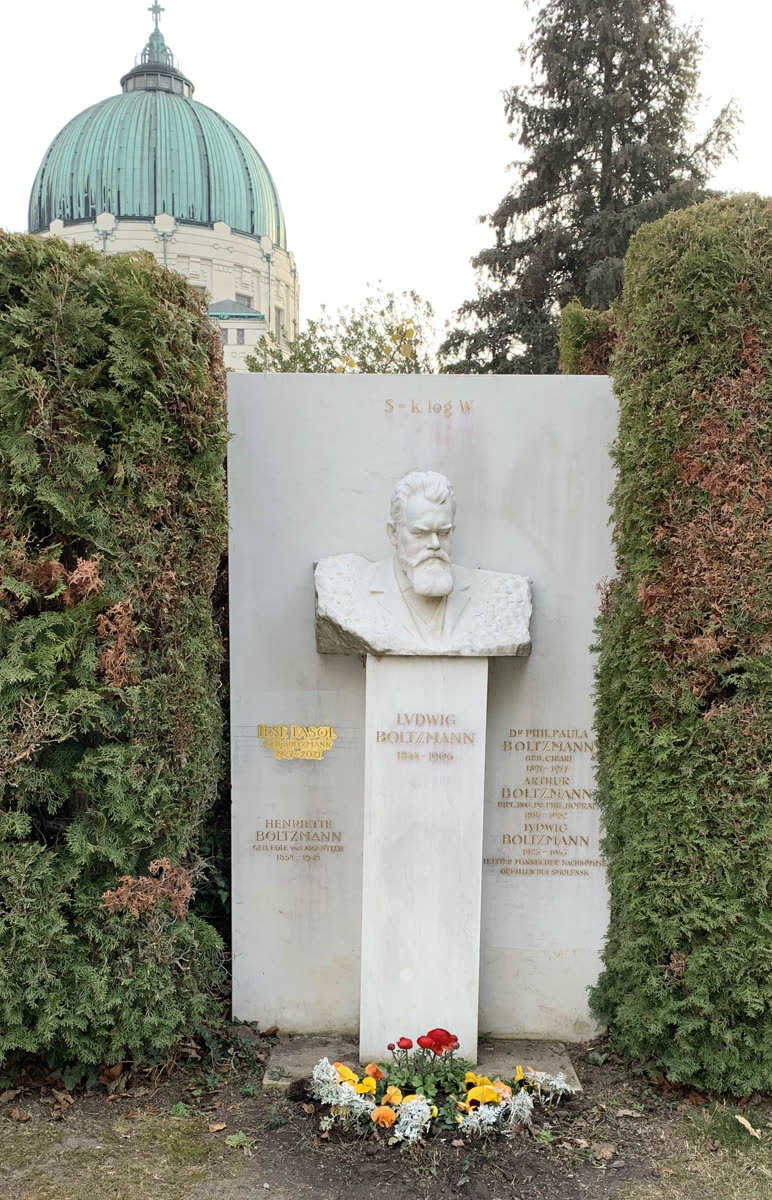
\includegraphics[width=\linewidth]{images/book4/boltzmann-grave.jpg}\par
{\footnotesize La tumba de Boltzmann.}
\end{minipage}
\end{history}

\section{Ejercicios}

\begin{exercise}[$\star$]\label{exo:b3:partition-functions:1}
Cuatro osciladores comparten cuatro cuantos. Enumérense las distribuciones, dese el peso de
cada una y compruébese que suman el número de maneras de colocar cuatro
cuantos \omterm{def:b3:many-electron-atoms:indistinguishable}{indistinguibles} en cuatro osciladores, $\binom{7}{3}$. ¿Qué distribuciones son las
más probables?
\end{exercise}

\begin{exercise}[$\star$]\label{exo:b3:partition-functions:2}
Dos niveles no degenerados están separados \qty{2.5}{kJ/mol}. Calcúlese la razón de sus
\omterm{def:b3:partition-functions:boltzmann}{poblaciones} a \qty{298.15}{K} y a \qty{1000}{K}. ¿Cuál es el límite a temperatura muy
alta?
\end{exercise}

\begin{exercise}[$\star$]\label{exo:b3:partition-functions:3}
% ledger: aw:Ar
Calcúlese la \omterm{def:b3:partition-functions:thermal-wavelength}{longitud de onda térmica} de un átomo de argón a \qty{298.15}{K} y su
función de partición de traslación en un volumen de \qty{1}{dm^3}.
\end{exercise}

\begin{exercise}[$\star$]\label{exo:b3:partition-functions:4}
% ledger: diat:N2.Be, diat:N2.ae, diat:HCl.Be, diat:HCl.ae
Con $B_0 = \qty{1.990}{cm^{-1}}$ (\ce{N2}) y \qty{10.440}{cm^{-1}} (\ce{H^{35}Cl}), calcúlense $\theta_{\mathrm R}$ y la
función de partición de rotación de alta temperatura de cada molécula a
\qty{298.15}{K}.
\end{exercise}

\begin{exercise}[$\star\star$]\label{exo:b3:partition-functions:5}
% ledger: diat:I2.we, diat:I2.wexe, diat:N2.we, diat:N2.wexe
Los números de onda fundamentales de \ce{I2} y \ce{N2} son \qty{213.27}{cm^{-1}} y
\qty{2329.92}{cm^{-1}}. Calcúlense $\theta_{\mathrm V}$, $q^{\mathrm V}$ a \qty{298.15}{K} y la fracción de moléculas
que no están en $v = 0$.
\end{exercise}

\begin{exercise}[$\star\star$]\label{exo:b3:partition-functions:6}
% ledger: diat:NO.split, lev:Cl.2P1_2
Calcúlese la función de partición electrónica a \qty{298.15}{K} del \ce{NO} (dos niveles doblemente
degenerados separados \qty{119.73}{cm^{-1}}) y del átomo de cloro (nivel fundamental ${}^2P_{3/2}$,
${}^2P_{1/2}$ a \qty{882.35}{cm^{-1}}). ¿Qué fracción de las moléculas de \ce{NO} está en
el nivel superior? ¿Hacia qué tiende $q^{\mathrm E}(\ce{NO})$ a alta temperatura?
\end{exercise}

\begin{exercise}[$\star\star$]\label{exo:b3:partition-functions:7}
A partir de $q^{\mathrm T} = V/\Lambda^3$, dedúzcanse la energía interna y la capacidad calorífica a
volumen constante de un mol de gas ideal monoatómico, y evalúese $U - U(0)$ a
\qty{298.15}{K}.
\end{exercise}

\begin{exercise}[$\star\star$]\label{exo:b3:partition-functions:8}
% ledger: aw:Ar, s0:Ar_g
Úsese la ecuación de Sackur--Tetrode para calcular la entropía molar estándar del
argón a \qty{298.15}{K}; compárese con el valor tabulado,
\qty{154.846}{J.K^{-1}.mol^{-1}}. ¿Cuánto cambia si la presión se divide por 10?
\end{exercise}

\begin{exercise}[$\star\star$]\label{exo:b3:partition-functions:9}
% ledger: diat:HCl.Be, diat:HCl.ae
Calcúlese la contribución de rotación a la entropía molar estándar de
\ce{H^{35}Cl} a \qty{298.15}{K} ($\theta_{\mathrm R} = \qty{15.02}{K}$).
\end{exercise}

\begin{exercise}[$\star\star\star$]\label{exo:b3:partition-functions:10}
Tratando $J$ como continuo, demuéstrese que el nivel de rotación más poblado de una
molécula lineal está cerca de $J_{\max} = \sqrt{T/2\theta_{\mathrm R}} - \frac12$. Evalúese para \ce{HCl}
($\theta_{\mathrm R} = \qty{15.02}{K}$) y \ce{CO} ($\theta_{\mathrm R} = \qty{2.766}{K}$) a \qty{300}{K}. ¿Por qué las dos
ramas de una banda infrarroja son más intensas a unas pocas rayas del centro?
\end{exercise}

\begin{exercise}[$\star\star\star$]\label{exo:b3:partition-functions:11}
% ledger: diat:H2.Be, diat:H2.ae
La fórmula de Euler--Maclaurin da $\sum_{J\ge0}f(J) \approx \int_0^\infty f(J)\dd J + \frac12f(0) -
\frac1{12}f'(0)$. Aplíquese a $f(J) = (2J+1)\eu^{-\theta J(J+1)/T}$ y demuéstrese que $q^{\mathrm R} \approx T/\theta +
\frac13$. ¿Para qué temperaturas es correcta $T/\theta$ al 1\,\%? ¿Es aceptable para \ce{H2}
($B_0 = \qty{59.32}{cm^{-1}}$) a \qty{298.15}{K}?
\end{exercise}

\begin{exercise}[$\star\star\star$]\label{exo:b3:partition-functions:12}
% ledger: diat:I2.we, diat:I2.wexe
Demuéstrese que la entropía molar de vibración tiende a cero cuando $T \ll \theta_{\mathrm V}$ y a
$R[1 + \ln(T/\theta_{\mathrm V})]$ cuando $T \gg \theta_{\mathrm V}$. Evalúense la expresión exacta y este
límite para \ce{I2} ($\theta_{\mathrm V} = \qty{306.9}{K}$) a \qty{298.15}{K}, y coméntese.
\end{exercise}

\section{Problema: contar la entropía del nitrógeno}

\begin{problem}[{Problema de fin de semana --- contar la entropía del nitrógeno: las
contribuciones de traslación, rotación, vibración y electrónica a su
entropía estándar, calculadas a partir de su espectro y comparadas con la tabla}]
\label{pb:b3:partition-functions:1}
% ledger: aw:N, diat:N2.Be, diat:N2.ae, diat:N2.we, diat:N2.wexe, s0:N2_g, const:h, const:kB, const:NA, const:c
El nitrógeno es el gas principal del aire. Su entropía molar estándar a
\qty{298.15}{K} se calcula aquí a partir de su masa molar, \qty{28.014}{g/mol}, y de sus
constantes espectroscópicas: $B_e = \qty{1.998241}{cm^{-1}}$, $\alpha_e = \qty{0.017318}{cm^{-1}}$, $\omega_e =
\qty{2358.57}{cm^{-1}}$, $\omega_ex_e = \qty{14.324}{cm^{-1}}$; su término electrónico fundamental es ${}^1\Sigma_g^+$.
Presión estándar $p^\circ = \qty{1}{bar}$; $k = \qty{1.380649e-23}{J/K}$, $h = \qty{6.62607015e-34}{J.s}$.

\medskip\noindent\textbf{Parte I --- Traslación.}
\begin{enumerate}
  \item Calcúlese la masa de una molécula.
  \item Calcúlese su \omterm{def:b3:partition-functions:thermal-wavelength}{longitud de onda térmica} a \qty{298.15}{K}.
  \item Calcúlese el volumen disponible por molécula, $kT/p^\circ$.
  \item Dedúzcase $q^{\mathrm T}/N$ y coméntese su magnitud.
  \item Calcúlese la entropía molar de traslación.
  \item ¿Cuánto cambiaría a la mitad de la presión?
\end{enumerate}

\medskip\noindent\textbf{Parte II --- Rotación.}
\begin{enumerate}[resume]
  \item Calcúlese $B_0$.
  \item Calcúlese $\theta_{\mathrm R}$.
  \item Dese el \omterm{def:b3:partition-functions:symmetry-number}{número de simetría} y dígase de qué da cuenta.
  \item Calcúlese $q^{\mathrm R}$ a \qty{298.15}{K}.
  \item ¿Está justificada la forma de alta temperatura?
  \item Calcúlese la entropía molar de rotación.
  \item Sin tener en cuenta los pesos de espín nuclear, ¿qué nivel de rotación es el más
        poblado?
\end{enumerate}

\medskip\noindent\textbf{Parte III --- Vibración y estados electrónicos.}
\begin{enumerate}[resume]
  \item Calcúlese el cuanto de vibración $G(1) - G(0)$.
  \item Calcúlese $\theta_{\mathrm V}$.
  \item Calcúlese $q^{\mathrm V}$ a \qty{298.15}{K}.
  \item ¿Qué fracción de las moléculas está en $v = 1$?
  \item Calcúlese la entropía molar de vibración.
  \item ¿Cuál es la contribución electrónica? ¿Por qué pueden ignorarse los estados electrónicos
        excitados?
\end{enumerate}

\medskip\noindent\textbf{Parte IV --- Suma y comparación.}
\begin{enumerate}[resume]
  \item Súmense las contribuciones.
  \item Compárese con el valor tabulado, \qty{191.609}{J.K^{-1}.mol^{-1}}.
  \item ¿En qué medidas se basa el valor calorimétrico de una tabla?
  \item ¿Por qué pueden las tablas dejar fuera el espín nuclear?
  \item Enúnciese el resultado: la entropía molar estándar del nitrógeno a \qty{298.15}{K}
        calculada a partir de sus constantes espectroscópicas.
\end{enumerate}
\end{problem}
